% %%%%%%%%%%%%%%%%%%%%%%%%%%%%%%%%%%%%%%%%%%%%%%%%%%%%%%%%%%%%%%%%%%%%%%%%%%%%%%%%%%%%%%%%%%%%%%%%%%%%
% %%%%%%%%%%%%%%%%%%%%%%%%%%%%%%%%%%%%%%%%%%%%%%%%%%%%%%%%%%%%%%%%%%%%%%%%%%%%%%%%%%%%%%%%%%%%%%%%%%%%
% SPACEFRAME
% %%%%%%%%%%%%%%%%%%%%%%%%%%%%%%%%%%%%%%%%%%%%%%%%%%%%%%%%%%%%%%%%%%%%%%%%%%%%%%%%%%%%%%%%%%%%%%%%%%%%
% %%%%%%%%%%%%%%%%%%%%%%%%%%%%%%%%%%%%%%%%%%%%%%%%%%%%%%%%%%%%%%%%%%%%%%%%%%%%%%%%%%%%%%%%%%%%%%%%%%%%

\graphicspath{{./\figurefolder/5SpaceFrame/}}

% ----------------------------------------------------------------------------------------------------
% 0. Front Matter
% ----------------------------------------------------------------------------------------------------
\chapter{Cooperative Robotic Scaffold-Free (Dis)Assembly of Triangulated Space Frames Designed with Rigidity Theory} \label{chap:5_SpaceFrame}

\thispagestyle{empty}

\vfill 
\section*{\normalsize\textmd{This chapter is primarily based on the following publication:}}
    \vspace{-0.3cm}
    \textbf{Bruun, E. P. G.}, Adriaenssens, S., \& Parascho, S. (2022). Structural rigidity theory applied to the scaffold-free (dis)assembly of space frames using cooperative robotics. Automation in Construction, 141, 104405. https://doi.org/10.1016/j.autcon.2022.104405

\section*{\normalsize\textmd{Contributor roles in publication:}}
    \vspace{-0.3cm}\noindent
    - Bruun: Conceptualization, Methodology, Software, Validation, Investigation, Writing (Original Draft), Writing (Review and Editing), Visualization\\
    - Parascho: Resources, Writing (Review and Editing), Supervision, Funding Acquisition \\
    - Adriaenssens: Writing (Review and Editing), Supervision, Funding Acquisition \\


% \section*{\normalsize\textmd{Acknowledgements:}}
%     \vspace{-0.3cm}
%     This research was partially developed through the Remote Robotic Assemblies Workshop that the author of this dissertation hosted at the 2021 ACADIA conference in collaboration with: Stefana Parascho, Gonzalo Casas, Beverly Lytle.

    \newpage
    \begin{figure}[ht]
        \centering
        \includegraphics [trim={0cm 0cm 0cm 0cm},clip,width=0.90\textwidth]{_cover_structure}
        \caption{A snapshot from the cooperative robotic assembly of a space frame arch structure.}
        \label{fig:chapter5_title}
    \end{figure} 

\section*{Abstract}
    This chapter presents a fabrication-informed design method for triangulated space frame structures that remain stable during all phases of their robotic assembly and disassembly without requiring external scaffolding. A graph theoretic framework, based on rigidity theory, is developed to allow the structure, its support conditions, and the impact of robotic support constraints to be simultaneously represented in a single topological framework. The structural system is sequentially designed with an assembly logic based on Henneberg graph-construction steps, which are executed with two robots through a cooperative rigidity-preserving sequence. Ensuring planarity of the resulting graph during these construction steps is shown to lead to intrinsic disassembly potentials within the system. A graph-based algorithm is presented to locate, isolate and remove locally rigid tetrahedral cells formed in the structural system. This algorithm is then utilized to compute a rigidity-preserving robotic disassembly sequence. The method is demonstrated in the design of a space frame arch structure (shown in \cref{fig:chapter5_title}) that is robotically (dis)assembled. 



% ----------------------------------------------------------------------------------------------------
% 1. Introduction
% ----------------------------------------------------------------------------------------------------
\newpage
\section{Introduction}\label{1_intro}
    Traditionally, architects and structural engineers place emphasis on the preliminary design of a structure in its finished state \citep{sharif_bim_2015}, but rarely account for the relationship between structural form and the resulting construction sequence that is necessary to reach this finished state. This can result in an expensive, time-consuming, or materially wasteful construction process. Construction costs can be substantial -- for example, formwork amounts to about 40\% of the total cost for reinforced concrete thin shells \citep{meyer_concrete_2005}. Looking at the other end of the building life-cycle, a structure is rarely designed with considerations for its efficient disassembly and potential reuse as a means to mitigate the large amount of waste construction activities currently contribute to landfill volumes \citep{zimmann_circular_2016}. Such a wasteful single-use design philosophy serves as a negative multiple on the high embodied energy associated with resource extraction and material processing requirements for building components \citep{kaethner_embodied_2012}. Technological developments to improve construction efficiency and material usage can help address some of these environmental impacts. The challenge is that the Architecture, Engineering and Construction (AEC) industry lags other industries when it comes to leveraging contemporary automation techniques and the associated productivity and environmental benefits \citep{barbosa_reinventing_2017}.
    
    The motivation behind this research is thus to aid in addressing the waste generation and productivity gap in the construction industry \citep{lu_framework_2011}, specifically when considering geometrically complex truss and space frame structures. This is accomplished through the development of a structural design framework for efficient construction using a cooperative robotic fabrication setup. Efficiency, in the context of fabrication, is herein defined as maintaining stability without requiring external formwork or scaffolding during all stages of assembly or disassembly. This framework thus addresses the AEC industry challenges by both improving construction productivity through automation, reducing construction waste by eliminating the need for temporary support material, and planning for disassembly of the structure. Planning for disassembly as a core consideration in the design process provides opportunities for future structural reconfiguration and reuse \citep{brutting_design_2019, brutting_optimum_2020, brutting_design_2021}.
    
    Industrial robots are applicable to architectural fabrication setups for discrete element structures due to their application versatility \citep{bravo-palacios_one_2020} and spatial precision in picking and placing material \citep{eversmann_robotic_2017}. They are also experiencing growing adoption in both industry and academic contexts \citep{ifr_world_2018} and are promising tools to tackle the AEC industry's lagging productivity and labor efficiency \citep{garcia_de_soto_productivity_2018, kumar_robotics_2016}. This chapter presents a \textit{fabrication-informed} design framework, which is defined as a framework where the structural design directly accounts for how the structure will be built and taken apart, in this case utilizing the capabilities of a robotic setup (specifically with respect to sequencing). This constitutes a departure from a more traditional linear approach to construction, where a robot would act as a generic tool at the end of the workflow to materialize a structure designed in a separate design phase. On the otherhand, a \textit{fabrication-informed} framework specifically developed for a cooperative robotic setup, in this chapter incorporates the multiple complimentary functions possible when several robots are working together: either placing members (during assembly) or removing parts of the structure (during disassembly), while also supporting the structure in its temporary state  \citep{parascho_cooperative_2019}.
    
    The proposed design method utilizes a graph-theoretic approach, based on rigidity theory, to link cooperative robotic construction with structural topology. This approach allows for the design of structures that have intrinsic scaffold-free assembly and disassembly potentials built directly into their preliminary design formulation.
    

\subsection{Chapter Organization}
    \Cref{sec:2_litreview} begins with a literature review on cooperative robotic fabrication and graph theory for the analysis of structural rigidity, followed by a more detailed explanation in \Cref{sec:3_spaceframes} of the specific concepts from rigidity theory that are necessary when representing bar and joint frameworks (i.e., trusses and space frames). \Cref{sec:4_assembly} presents a topology-driven design method for structures that can be assembled with cooperating robots in a rigidity-preserving manner. \Cref{sec:5_disassembly} then presents a graph-based algorithm that is used to plan a rigidity-preserving cooperative robotic disassembly sequence for the same structure. The method is demonstrated in the design of a spanning wooden space frame arch structure, with a discussion of the results from its physical assembly and disassembly presented in \Cref{sec:6_results}. The chapter concludes in \Cref{sec:7_conclusion}.

% ----------------------------------------------------------------------------------------------------
% 2. Literature Review
% ----------------------------------------------------------------------------------------------------  
\section{Literature Review} \label{sec:2_litreview}

\subsection{Cooperative Robotic Fabrication in Construction} \label{sec:2__robotfab}
    In the AEC industry, industrial robotic arms were first applied to the construction of modular homes  \citep{bock_construction_2007, bock_future_2015} and then in single-purpose automation systems \citep{albus_trip_1986, cousineau_construction_1998, huang_factor_1990, ueno_construction_1986}. Since their first adoption, robotic systems have continued to improve their functionality in unstructured environments \citep{bock_site_2016, skibniewski_robotics_1989}, which has substantially improved their viability in the construction of structures with complex geometries \citep{davila_delgado_robotics_2019}.
    
    Growth in the field of digital fabrication (dfab) saw the first large-scale explorations in an architectural context of robots applied to the construction of geometrically complex structures \citep{gramazio_digital_2008, gramazio_made_2014, kohler_programmed_2014}. At the outset, robots were used to build prefabricated load-bearing but non-standardized undulating walls made of discrete volumetric elements \citep{bonwetsch_informed_2006, bonwetsch_digitally_2007, kohler_gantenbein_2014}, followed by the DFAB house \citep{empa_dfab_2021} as an example of how digital design and robotic fabrication processes can be used to build different non-standardized components and assembled in a structure \citep{willmann_robotic_2016, hack_mesh_2017, hack_structural_2020}. Yet despite these advancements, when specifically applied to the construction of discrete element structures, robotic fabrication is still predominantly utilized for the construction of vertical layer-based structures \citep{bartschi_wiggled_2010,kohler_gantenbein_2014, bonwetsch_informed_2006, bonwetsch_digitally_2007, piskorec_brick_2018, dorfler_mobile_2016, giftthaler_mobile_2017}. A review of recent trends in multi-agent fabrication, applied in a collaborative (human-robot) or cooperative (robot-robot, cobot) framework, shows how multi-agent approaches can help to expand the feasible design space of robotic fabrication \citep{han_bridging_2021, petersen_review_2019, braganca_brief_2019}.
    
    Maintaining stability and mitigating unwanted forces and deflections during construction can prove a significant challenge when using additive fabrication processes \citep{bruun_three_2021, carneau_additive_2020, motamedi_supportless_2019}. This can be a limitation to the design freedom of discrete element structures realized with robotic fabrication methods. One solution to the challenge of maintaining stability is to work with specially designed discrete elements that allow some level of interlocking to provide local stability during construction \citep{latteur_droxel_2022,goessens_feasibility_2018}. Another approach is to utilize a cooperative robotic fabrication strategy (i.e., multiple robots working together to perform a task that cannot be performed with one robot alone), which can lead to new self-supporting construction processes, a concept proposed for space frame construction by Parascho \citep{parascho_cooperative_2017, parascho_computational_2018, parascho_cooperative_2019}. In Parascho's work, structural stability during construction was achieved without scaffolding by designing the structure specifically for fabrication using two robots sequenced in a cooperative manner. The robots take turns performing either the function of: (1) picking up and accurately placing structural components, or (2) holding and providing temporary support over indefinite periods of time to a partially completed structure. These are tasks that a human would struggle with but are well-suited to a robotic agent. Thus, these structures  were only realizable in a self-stable way (i.e., without external scaffolding) when explicitly leveraging the use of multiple robots.

    The support/place approach has been used in a number of subsequent cooperative robotic fabrication projects to construct complex discrete element structural forms in a range of materials and scales. For example, the fabrication of non-planar timber modules, where cooperating robots were used as a way to minimize the need for scaffolding in the intermediate stages of fabrication \citep{thoma_robotic_2018}. Several geometrically complex spanning structures have also been constructed without scaffolding using a cooperative robotic strategy: a bifurcating arch structure built out of foam blocks \citep{wu_robotic_2018}, and a doubly-curved brick shell \citep{parascho_robotic_2020, parascho_lightvault_2021, han_concept_2020}, and a branching tree structure \citep{bruun_humanrobot_2020}. In general, the trend of moving from single to multiple agents for collaborative processes increases the complexity of the relationship between fabrication sequence and structural design. It is thus necessary to develop a design framework that can handle the increasing complexity of setups with multiple robots working together.   
    
\subsection{Graph Theory and Structural Isomorphism}\label{sec:2__graphs}
    Designing a discrete element structure for stability during assembly and disassembly requires a numerical formulation that characterizatizes this objective. The goal is to integrate the fabrication sequence with the structural design, while considering the interaction of the multiple robotic agents without an overly prescriptive method that stiffles geometric exploration and creativity in the preliminary design. These objectives are formulated here as a topological problem: relating the connection between the structural elements and the structural stability during construction, while taking into account the potential of utilizing robotic support.
    
    A topological problem can be expressed as a graph, $G = (V,E)$, which is a discrete mathematical structure in $\mathbb{R}^2$ made up of vertices, $V$,  connected by edges, $E$, that represent pairwise relations between objects. The foundations of graph theory (i.e., the study of such structures) were laid by Euler in his solution to the \textit{Seven Bridges of Köningberg} problem \citep{euler_solutio_1758}. Graph theory has since seen broader application in the study of topology and in applied science applications to model how objects are distributed and connected in complex systems including circuits \citep{kirby_what_2016, kirchhoff_ueber_1847}, elastic networks \citep{kron_elastic_1962}, and structures \citep{fenves_network-topological_1963, fenves_structural_1966, lind_analysis_1963}. More recently, topological representations have also been used in geometric form-finding methods \citep{block_thrust_2007, ohlbrock_computer-aided_2020, pastrana_constrained_2021}.
    
    A graph is isomorphic to a physical system if it has a one-to-one mapping with the elements in the system it represents. Given such a representation, one can determine properties of the underlying system with graph theoretic approaches based only on topological information \citep{shai_isomorphic_1999}. The general principle is that certain properties of the graph represent the intrinsic physical behavior of the system it represents. Isomorphic graphs have thus been used to show parallels in the analysis and formulation of a broad class of physical systems such as: trusses, dynamic mass-spring-damper oscillator systems, and planetary gear systems \citep{shai_representation_1998, shai_graph_1999, shai_isomorphic_1999}. In the context of bar and joint frameworks (i.e., trusses and space frames), this relationship between a graph and its isomorphic structure can be used to compute force and displacement quantities \citep{kaveh_structural_1992, kaveh_role_2005, shai_representation_1998} or generic properties such as rigidity and stability \citep{shai_isomorphic_1999}.
    
    
\subsection{Infinitesimal Rigidity and the Laman Count Condition} \label{sec:2__laman}
    For a bar and joint framework, a necessary condition for infinitesimal rigidity was first formulated by Maxwell as a counting rule relating the number of nodes, $v$, to the number of members, $e$, in the framework. A structure needs a minimum of $e = 2v - 3$ members in $\mathbb{R}^2$, and a minimum of $e =3v - 6$ members in $\mathbb{R}^3$ to be infinitesimally rigid \citep{maxwell_calculation_1864}. An infinitesimally rigid structure is one where every infinitesimal motion is a Euclidean one (i.e., a rigid body motion); a structure is infinitesimally rigid iff it is statically rigid, meaning that every equilibrium load has a resolution \citep{tay_generating_1985}. The relationship between the number of nodes and members was later refined by Calladine to characterize the number of mechanisms present in a framework \citep{calladine_buckminster_1978, connelly_when_2009}. However, the overall Maxwell count condition is a necessary, but not sufficient, condition for infinitesimal rigidity. This is demonstrated with the two trusses in \Cref{fig:fig1_trusses}, where both satisfy the count condition but only the right one is infinitesimally rigid. Thus, a more generalized approach, based on rigidity theory (a branch of graph theory), is necessary to determine if a bar and joint framework is rigid based on the topology of its isomorphic graph.
    
    \begin{figure}[ht]
    	\centering
    	\includegraphics [trim={0cm 0cm 0cm 0cm}, clip, width=0.99\linewidth]{fig1_trusses}
    	\caption{Two trusses that both satisfy the planar Maxwell count condition but only the right is infinitesimally rigid.}
    	\label{fig:fig1_trusses} 
    \end{figure}    
    
    If for a graph, $G = (V,E)$, where the number of edges is $|E| = 2|V| - 3$, every subgraph, $G = (V',E')$, satisfies the count condition, $|E'| \le 2|V'| - 3$, then the graph is minimally rigid (i.e., infinitesimally rigid with the least amount of edges possible). Theorem 5.6 of Laman’s paper \citep{laman_graphs_1970} proved that this condition is not only necessary, but also sufficient, for a graph to be generically minimally rigid in the plane. The term \textit{generic}, in reference to rigidity, refers to a graph that has at least one isomorphic realization (i.e., a specific mapping of vertices to physical nodes corresponding to a truss structure) that is statically rigid \citep{tay_generating_1985}. This theorem, when applied to the cases shown in \Cref{fig:fig1_trusses}, correctly identifies the 6-noded truss on the right as statically rigid with the minimum required 9 members. A sub-graph counting condition, with $|E'| \le 3|V'| - 6$ instead, can also be used to determine if a graph is generically minimally rigid with respect to realizations in $\mathbb{R}^3$. These principles can be used to build generically rigid graphs, which thus have at least one isomorphic realization as a space frame in $\mathbb{R}^3$ that is isostatic (i.e., statically rigid and infinitesimally rigid). This procedure, and certain caveats, are further explained in \Cref{sec:3_spaceframes}.
    

\subsection{Research Contributions} \label{sec:2__contribution}
    This research extends past work on the scaffold-free cooperative robotic fabrication of space frames \citep{parascho_cooperative_2019} by redefining the design process and assembly logic through a novel graph theoretic framework based on rigidity theory. A spatial structure is represented as its isomorphic graph \citep{shai_isomorphic_1999}, where the structural topology and influence of robotic support is simultaneously evaluated from the perspective of preserving rigidity in the graph. The topology-driven design method developed using this framework is able to unify the generation of a space frame geometry with the criteria that the resulting structure has a feasible scaffold-free assembly and disassembly sequence. The design method is also considered \textit{fabrication-informed} since the resulting structure is directly designed based on what is possible when sequencing two robots in a cooperative manner. The following is a summary of the main contributions of the research presented in this chapter:
    
    \begin{itemize}
        \item Presentation of the isomorphic \textit{stability graph} as a unified framework to represent a structure and its supports, and the impact of robotic support on the rigidity of a graph.
        \item Recontextualization of an existing cooperative robotic assembly sequence for space frames \citep{parascho_cooperative_2019} through the lens of rigidity-preserving Henneberg assembly steps used for the mathematical construction of rigid graphs.  
        \item Development of a sequential topology-driven design method that links physical assembly and disassembly with the properties of graph planarity and minimal rigidity. These properties, resulting in a structure comprised of locally rigid tetrahedral cells, are used to guarantee that a scaffold-free assembly (member-by-member) and disassembly (cell-by-cell) sequence exist for the structure. 
        \item Demonstration of the proposed method in the design of a space frame arch structure, and implementation of a cooperative robotic sequence for both its scaffold-free assembly and disassembly.
    \end{itemize}
     


% ----------------------------------------------------------------------------------------------------
% 3. Space Frames as Graphs
% ----------------------------------------------------------------------------------------------------
\section{Graph Representation for Space Frame Structures}\label{sec:3_spaceframes}
    This section expands the general principles of rigidity theory and structural isomorphism introduced in \Cref{sec:2__graphs,sec:2__laman} with specific concepts that are required to represent a space frame structure as a graph. This representation forms the basis for the design method that guarantees a rigidity-preserving assembly and disassembly sequence. The following topics are covered: Henneberg assembly steps to build generic minimally rigid graphs isomorphic to 3D bar and joint frameworks  (\cref{sec:3__henneberg}), representing a minimally rigid tetrahedral building block (or cell) as a graph (\cref{sec:3__tetrahedral}), and accounting for structural supports and evaluating their impact on rigidity through a stability graph representation (\cref{sec:3__supports}).
    
    The terms \textit{vertex} and \textit{edge} are used when referring to a graph, which is a representation that lives in $\mathbb{R}^2$, and \textit{node} and \textit{element} are used when referring to an \textit{realization} or \textit{physical \ embedding} (used interchangeably) of the graph in $\mathbb{R}^2$ (i.e., a truss) or $\mathbb{R}^3$ (i.e., a space frame). The term \textit{rigidity} will also henceforth be used to refer to \textit{generic infinitesimal rigidity} unless noted otherwise.

\subsection{Constructing Rigid Graphs: Henneberg Assembly Steps} \label{sec:3__henneberg}
    While the Laman condition provides a definitive way to check rigidity in the plane ($\mathbb{R}^2$), its naïve algorithmic implementation results in an exponential time algorithm \citep{shai_isomorphic_1999}. Modern algorithms exist that reduce the complexity of verifying minimal rigidity to polynomial \citep{grotschel_ellipsoid_1981,gortler_characterizing_2010}, quadratic \citep{jacobs_algorithm_1997,bereg_certifying_2005}, or even sub-quadratic \citep{daescu_towards_2009} time. However, these algorithms can be complex to implement. But rigidity can for large and complex graphs be more easily checked through a particular graph's sequential assembly sequence (if this information is available), since every minimally rigid graph can be built up starting from a single edge using only a simple set of rules. This process is named after Henneberg, who first introduced the idea of preserving rigidity in the plane by sequentially aggregating a low-valent vertex to the existing graph \citep{henneberg_graphische_1908}. Thus, if a larger graph is found to be the result of a series of rigidity-preserving Henneberg steps then by inductive reasoning it is guaranteed to be rigid itself.
    
    Extending this concept to graphs embedded in space ($\mathbb{R}^3$), starting from a $C_3$ graph (i.e., 3-vertex cycle) with non-collinear embedding, every minimally rigid graph can be built up through a sequence of the following three Henneberg assembly steps \citep{tay_generating_1985}, illustrated in \Cref{fig:henneberg}:
    
    \setlist[itemize]{leftmargin=0.5in, align = right}
    \begin{itemize}
        \item [Type 1:] (i) add a new vertex, (ii) connect the new vertex to any 3 vertices in the graph.
        \item [Type 2:] (i) delete any edge, (ii) add a new vertex, (iii) connect the new vertex to the 2 vertices incident to the deleted edge, (iv) connect the new vertex to any 2 other vertices in the graph.
        \item [Type 3a:] (i) delete any 2 edges, (ii) add a new vertex, (iii) connect the new vertex to the 4 vertices incident to the deleted edges, (iv) connect the vertex to any other vertex in the graph.
        \item [Type 3b:] (i) delete any 2 edges, (ii) add a new vertex, (iii) connect the new vertex to the 3 vertices incident to the deleted edges, (iv) connect the vertex to any 2 other vertices in the graph.
    \end{itemize}
    
    \begin{figure}[ht]
    	\centering
    	\includegraphics [trim={0cm 0cm 0cm 0cm}, clip, width=0.99\linewidth]{fig0_henneberg_3D} %tight
    	\caption{Henneberg assembly steps for the construction of a graph with a generic rigid embedding in space ($\mathbb{R}^3)$}
    	\label{fig:henneberg} 
    \end{figure}    

    Only after executing a Type 1 or Type 2 step is the resulting graph guaranteed to be a generically minimally rigid (i.e., it has at least one possible rigid realization in space). A Type 3 step has been shown to result in a graph without a rigid realization in some special cases \citep{tay_generating_1985,grasegger_realizations_2018, grasegger_lower_2020}. The failure of Type 3 steps to definitively preserve rigidity is related to the fact that the Laman condition is a necessary, but not sufficient condition, for a minimally rigid graph embedded in space, as shown by the \textit{double banana} counter-example in the literature \citep{cheng_nucleation-free_2009, pollaczekgeiringer_uber_1927}. Providing a combinatorial characterization of rigidity in space, as exists in the plane, is a major open problem in graph theory \citep{cruickshank_spaces_2014}. This issue can be mitigated through imposing additional topological and geometric constraints on the resulting physical structure that the graph is isomorphic to. For example, explicitly avoiding the formation of an axis of rotation in the \textit{double banana} structure. Another way to preserve the property of rigidity in the overall graph is to construct the graph through the aggregation of smaller sub-graphs (referred to here as cells) with proven rigid realizations.
    
    Thus, the design method presented in this chapter is based on a strictly Type 1 assembly logic, which is guranteed to preserve rigidity. But using Type 2 or 3 Henneberg steps for assembling rigid structures is a possible foundation for the development of bi-directional (i.e., both adding and removing elements) fabrication sequences for more topologically varied structures.
    
\subsection{The Tetrahedral Cell as a Rigid Building Block} \label{sec:3__tetrahedral}
    The tetrahedron, which can be represented with a skeletal framework of 4 nodes and 6 elements, is the simplest platonic solid and corresponds to a minimally rigid cell from which larger rigid structures can be assembled. Due to their geometric simplicity, they are used as the fundamental building block for space frame structures designed to be assembled and disassembled with the cooperative robotic method described in this chapter. More complex rigid cells, composed of more vertices, could also be used in this method, but their stability-preserving assembly feasibility is contingent on the number of robotic agents available in the setup.
    
    The graph representing the topology of a tetrahedron is minimally rigid, with generic rigid realizations in $\mathbb{R}^3$ under the geometric constraint that no three nodes are collinear and that all four nodes are not coplanar \citep{tay_generating_1985}. Based on inductive reasoning, these constraints, when coupled with the Laman count condition, are sufficient to guarantee rigidity in a structure that is built up from a collection of rigid tetrahedral cells. \Cref{fig:fig2_cell_rigidity} illustrates the isomorphic graph representation of such a cell as a planar realization (i.e., no edges crossing) of the $K_4$ graph, which is built from, $G_0 = C_3$, with a Henneberg Type 1 step: $G_1= (V_0\cup \{3\}, E_0 \cup \{e_2,e_3,e_4\})$. The resulting graph satisfies the Laman count requirements, has a valid Henneberg construction sequence characterization, and known rigid realizations in $\mathbb{R}^3$ under the geometric constraints mentioned above. The representation of a structure without support conditions, as in \Cref{fig:fig2_cell_rigidity}, is defined as a rigidity graph.
    
    Planarity is another important property of the graph of the tetrahedral cell, which will be discussed in the context of the assembly logic (\cref{sec:4__method}) and the disassembly sequence algorithm (\cref{sec:5__algorithm}). 
    
    \begin{figure}[ht]
    	\centering
    	\includegraphics [trim={0cm 0cm 0cm 0cm}, clip, width=0.99\linewidth]{fig2_cell_rigidity} %fully trimmed
    	\caption{Rigidity graph (right) and rigid realization (left) of a minimally rigid tetrahedral cell ($|V| = 4$, $|E| = 6$).}
    	\label{fig:fig2_cell_rigidity} 
    \end{figure}
    
\subsection{Structural Supports Represented in a Graph} \label{sec:3__supports}
    When representing a structure including its support conditions, its isomorphic graph is herein defined as a stability graph. For example, a structure might be rigid based on its topology but still undergo rigid-body motion based on its support conditions. One of the strengths of a topological approach is that the same methodology to assess rigidity, can be extended to evaluate stability based on the degrees of freedom (DOFs) being constrained at vertices in the graph. Thus, if the stability graph is found to be rigid (i.e., through the Laman count and Henneberg sequence characterization), then the structure it is isomorphic to is stable. This process is described for trusses ($\mathbb{R}^2$) in \citep{shai_isomorphic_1999} and extended to space frames ($\mathbb{R}^3$) in this chapter.
    
    A stability graph is built by representing the DOFs in the system as additional graph vertices, which - for a graph realized in $\mathbb{R}^3$- are the three translations in Euclidean space. Edges are then added between these support vertices and the vertices that represent structural nodes restrained in translation by a support. \Cref{fig:fig3_cell_stability} shows two different support conditions: (1) a single pin at the base of the structure, and (2) a base pin, roller, and directional pin (X \& Z). Condition (1) is unstable as the structure, one rigid tetrahedral cell, is free to rotate about its base. This rigid body motion can equivalently be proved by analysis on the graph representation: each supported DOF is shown as an edge in the graph, $E_{support}= \{a,b,c\}$, hence the global count for this graph is now 12, which does not satisfy the required global Laman count, 15. Condition (2) on the other hand is stable, with $E_{support}= \{a,b,c,d,e,f\}$, hence the total count is 15, which satisfies the global Laman count, 15. But for a stability graph to be generically rigid it must also satisfy certain constraints when considering realizations in $\mathbb{R}^3$, similar to how the rigidity graph of the tetrahedral cell must satisfy certain geometric constraints as discussed in \Cref{sec:3__tetrahedral}. If adjacent support edges are not independent this has the effect of removing a supported DOF from the system and destabilizing it. For example, in \Cref{fig:fig3_cell_stability}, if edges $\{e,f\}$ (i.e., $(z,2)$ and $(z,3)$) represent supports that are in the axis of member $(2,3)$ (i.e., the support forces are collinear), then the system would not be stable. Additionally, a minimum of three nodes in the structure must at any time have at least one DOF constrained, to prevent an axis of rotation forming. This result corresponds to the principles of statics, where every equilibrium load can only be resolved through the global equations of force and moment equilibrium when precisely 6 independent support reactions are acting in at least one plane.

    \begin{figure}[h]
    	\centering
    	\includegraphics [trim={0cm 0cm 0cm 0cm}, clip, width=0.95\linewidth]{fig3_cell_stability} %fully trimmed
    	\caption{Stability graphs representing two different sets of support conditions on the same minimally rigid space frame structure. Condition 1 (left) is unstable since $|E| = 12 < 3|V| - 6$, while condition 2 (right) is stable since $|E| = 15 \geq 3|V| - 6$, a Henneberg assembly sequence exists, and the geometric constraints specified in \Cref{sec:3__tetrahedral,,sec:3__supports} are satisfied. Vertices/nodes in red are supported.}
    	\label{fig:fig3_cell_stability} 
    \end{figure}
    
    Using this topological representation, unifying structure and support, the structure can be said to be stable if its stability graph is rigid. Minimal rigidity of the stability graph is verified through the same process as the for the graph of the structure, by showing that there exists a sequence, $S$, of Henneberg Type 1 or 2 steps ($h_1$ or $h_2$) to build the final graph, $G_n$, starting from a rigid graph, $G_0 = (V_0,E_0)$:
    
    \begin{equation}
        \exists \; S\{H_1\cdots H_n\} \ \text{s.t.} \ G_0\rightarrow G_n \ | \ H \in \{h_1,h_2\}
    \end{equation}
    	
    There may exist numerous valid Henneberg sequences, $S$. The stability graph, $G_3$, referring to support condition (2) in \Cref{fig:fig3_cell_stability}, can be built from the starting graph, $G_0$, referring to the graph of the tetrahedral cell in \Cref{fig:fig2_cell_rigidity}, through one such sequence:
    
    \begin{itemize}
        \item $H_1 = h_1$: $G_1 = (V_0\cup \{Z\},\ E_0 \cup \{c,e,f\})$
        \item $H_2 = h_1$: $G_2 = (V_1\cup\ \{Y\},\ E_1 \cup \{b,s_2,(Y,2)\})$
        \item $H_3 = h_2$: $G_3 = (V_2 \cup \{X\}, E_2 \setminus (Y,2) \land E_2 \cup \{a,d,s_1,s_3\})$
    \end{itemize}
	
	
% ----------------------------------------------------------------------------------------------------
% 4. Assembly
% ----------------------------------------------------------------------------------------------------
\section{Designing a Space Frame Structure for Cooperative Robotic Assembly} \label{sec:4_assembly}
     In this section, principles of graph rigidity, and their characterization through Henneberg assembly steps, are implemented to develop a topology-driven design method for the scaffold-free construction of space frame structures. The main objective is to design the structure explicitly considering a cooperative fabrication sequence with two robots \citep{parascho_cooperative_2019}. Thus, the structure's stability graph must remain rigid throughout the full assembly process while planarity must be preserved in the graph isomorphic to the structure. The property of planarity is shown to result in the formation of locally rigid cells arranged in a linear manner in the overall structure, which will be crucial in ensuring that a scaffold-free disassembly sequence is also embedded in the structural design. Thus, the design method is introduced through the lens of efficient rigidity-preserving assembly, but has explicit considerations for disassembly in its formulation.
     

\subsection{Cooperative Robotic Assembly Strategy} \label{sec:4__robotic_comp}
    The structural design method is based on a cooperative fabrication sequence with two robots ($R_1$ and $R_2$) that alternate their role in placing members and providing temporary support to the structure, as described in \citep[p.74-77]{parascho_cooperative_2019}. After placing a member, a robot is left supporting the structure, while the other robot is free to release the structure and retrieve and add the following member.
    
    The axial forces in individual members are resolved at concurrent points at the structural joints, illustrated for a system of three members in \Cref{fig:fig4_robotic_steps}. There is only one possible physical arrangement of members at the joint level for each spatial mapping of the vertices. As a result, there exists a true one-to-one relation between the graph and the load path in the realized structure. A translational restraint shown as an edge in the graph, also represents the resulting force equilibrium in this pin-joint when a support is acting on it. This relation only exists for an idealized bar and joint structure where axial forces are resolved at concurrent points, because a graph representation only carries information about the connection topology. Capturing more complex equilibrium conditions, such as moments in the connections, requires information about offsets and distances not present in a topological representation. For example, the joint-level load paths cannot be fully characterized in a reciprocal frame style connection system where numerous relative member placements are possible for the same joint (as in previous work \citep{parascho_cooperative_2017, parascho_computational_2018}).

    \begin{figure}[ht]
    	\centering
    	\includegraphics [trim={0cm 0cm 0cm 0cm}, clip, width=0.99\linewidth]{fig4_robotic_steps} %full trim
    	\caption{Cooperative robotic sequence to execute a 3-member rigidity-preserving Henneberg Type 1 step for members with concurrent lines of action at the added node. Stage B (left): $R1$ = Place, $R2$ = Support; Stage D (middle): $R1$ = Support, $R2$ = Place; Stage F (right): $R1$ = Place, $R2$ = Support (adapted \citep[fig. 3.19]{parascho_cooperative_2019})}
    	\label{fig:fig4_robotic_steps} 
    \end{figure}

    
\subsection{Robotic Support and Henneberg Assembly} \label{sec:4__robotic}
    In a structure constructed from concurrent members, according to a cooperative assembly strategy, the action of a temporary robotic support on the structure can be represented in the stability graph. The two vertices incident to the member a robot is supporting, are connected to the three graph vertices representing the translational constraints using the methodology described in \Cref{sec:3__supports} and shown during the execution of a Henneberg Type 1 step in \Cref{fig:fig14_robot_henneberg}. The robot thus affects the property of rigidity in the stability graph by altering the edge counts in the overall graph and its subgraphs.

    \begin{figure}[ht]
    	\centering
    	\includegraphics [trim={0cm 0cm 0cm 0cm}, clip, width=0.99\linewidth]{fig14_robot_henneberg} %full trim
    	\caption{The stability graphs at each of the 6 stages (A-F) for a Henneberg Type 1 step executed with two robots (R1 and R2) either supporting a member or retrieving the next member to add to the structure. Each edge highlighted in red represents three independent edges connecting a supported vertex in the structure to each of the three vertices representing the X, Y, Z translation constraints.}
    	\label{fig:fig14_robot_henneberg} 
    \end{figure}
    
    However, from the perspective of rigidity, despite utilizing the support provided by two robots during fabrication, there are limitations to the feasible sequence of adding members. For example, in a situation where elements are built off an existing rigid structure, but are placed without being incident to the same end node: one member can initially be placed and supported by either robot, but would later become unstable since it is only connected at one pinned end once the robot releases it to retrieve the next element. In the graph representation, this can be verified with a failure to achieve the global Laman count. One way to overcome this failure, is to add new members to the structure in mutually reinforcing ways (i.e., incident to the same new node) so that they assemble towards states of rigidity in the graph isomorphic to the structure. 
    
    Building towards stages of rigidity can be evaluated through the lens of Henneberg assembly steps. A Type 1 step requires an additional vertex to be connected to the graph at three distinct vertices to maintain rigidity. In an applied context, during physical construction, such a step cannot happen instantaneously, but is instead executed through the sequential placement of three separate members. This process is shown in \Cref{fig:fig14_robot_henneberg} through the stability graph representation at each of the 6 stages (placing and retrieving members) required to execute a full Henneberg sequence with two robots. The sequence starts with a generic rigid structure supported by a robot in stage A; for clarity the graph of the rest of the structure and its non-robotic foundation supports are not shown in \Cref{fig:fig14_robot_henneberg}. Each vertex that is supported by a robot at a stage is connected to the vertices representing the X, Y, Z translational support DOFs. During the first two member placements (stages B and D), there must be at least one robot supporting the partially completed Henneberg structure (i.e., the sub-structure of members connecting to the newly added node) for it to be rigid. Once the third and final member in the sequence is placed (stage F), the Henneberg step is complete, and the graph of the structure (in this case representing a simple tetrahedral cell) becomes minimally rigid without requiring robotic support. The aggregation process can then be repeated with the addition of another vertex to the existing graph, which is realized through the execution of another 3-member cooperative sequence with two robots. To compliment the graph representation in \Cref{fig:fig14_robot_henneberg}, the physical representation of such a sequence is illustrated in \Cref{fig:fig4_robotic_steps} for the member placement stages (B, D, F) in the process of adding a node to an existing rigid structure. Depending upon the type of external non-robotic foundation support, a robotic support to the structure might still be required to guarantee stability of the overall structure, even at the completion of a Henneberg step. It is possible for the rigidity graph to be rigid while the stability graph is not, as is the case for a structure supported on a single external base pin (i.e., Condition 1 in \Cref{fig:fig3_cell_stability}).  
    
    In \Cref{sec:3__supports} it was explained that a total of 6 DOFs, represented as 6 edges in the graph, must be constrained on a minimum of 3 vertices (i.e., embedded as a plane) for the stability graph to remain rigid. This requirement is satisfied in a 3-member Henneberg sequence as there is always at least one robot supporting the structure. Since the robot constrains the movement of two vertices incident to the member it supports, this provides more support than is strictly necessary for the minimally rigid criteria. For example, the stability graph in \Cref{fig:fig3_cell_stability} has 3 additional edges, $E = \{(Y,2),(Y,3),(X,3)\}$, if member $e_3$ was supported by a robot (i.e., $V_{support} = \{2,3\})$. But although such a structure would result in an over-constrained system (i.e., statically indeterminate), this over-constraining does not negatively impact the stability in the structure. Adding edges representing supports to a minimally rigid stability graph does not undermine its underlying property of rigidity; if a structure is stable under certain set of support conditions, additional supports only add to the structural redundancy of the system.
    

\subsection{Assembly Logic} \label{sec:4__approach}
    A structure is designed sequentially to reflect its order of assembly, where each new node is connected back to three existing nodes in the structure, as per a Henneberg Type 1 step, forming a triangulated configuration as in \citep[pg. 52-53]{parascho_cooperative_2019}. This assembly logic has been recontextualized and developed in this chapter through the graph-based analysis approach described in \Cref{sec:4__robotic_comp,,sec:4__robotic}, to show that the properties of rigidity can be preserved at both the local and global level when utilizing a cooperative robotic place/support strategy as illustrated in \Cref{fig:fig4_robotic_steps}. However, the assembly logic used here differs from previous work \citep{parascho_cooperative_2019} as a new node in the structure is further specified to always connect to three nodes on the most recently formed tetrahedral cell. This approach guarantees that a rigid tetrahedral cell is formed after each 3-member aggregation phase. Thus, each added member is guaranteed to be part of at least one rigid cell. This is equivalent to specifying that a new vertex must be added to the current graph such that the resulting graph has a 1) planar realization (i.e., can be drawn with no edges crossings), and 2) linear partial order (i.e., a collection of rigid cells in series). 
    
    The process of adding new nodes to three nodes on the most recently completed cell in the existing structure is not strictly necessary when just considering rigidity during assembly. But this aggregation logic becomes important when planning for a disassembly sequence as it guarantees the topological uniformity of the graph. The property of planarity and the linear partial order in the nested graph that is produced when utilizing the this assembly logic guarantees that an efficient stability-preserving cooperative robotic sequence can later be found for disassembly. Each member is guaranteed to be part of at least one rigid cell, which allows for an algorithmic process to locate, isolate, and remove these self-contained rigid cells during disassembly. This algorithm is explained in detail in \Cref{sec:5__algorithm}. Thus, a design process utilizing the assembly logic described in this section is considered fabrication-informed as it has considerations for not just efficient assembly, but also for ease of disassembly, built directly into its formulation.
    
    In contrast, if an assembly logic based on connecting to any three nodes is used, the structure can still be assembled without requiring support but is now not guaranteed to be composed of rigid cells. This case is illustrated in \Cref{fig:fig13_stefana_assembly}, where node 5 is connected to the existing structure with $E = \{(0,5),(3,4),(4,5)\}$. The result is a supergraph of the utility graph (UG), and is therefore non-planar \citep{trudeau_introduction_1994}. It is possible to find two $K_4$ subgraphs, which correspond to the existence of two tetrahedral cells, $C_1$ and $C_2$, in the original structure. But there is no such subgraph formed with the new edges in the graph, so no valid cell is formed when adding these members. A cell can be formed given the existing configuration by adding a single edge, $e = (0,4)$, or by swapping $e = (0,5)$ for $e = (1,5)$ as can be observed in \Cref{fig:fig13_stefana_assembly}. But in general, if such an assembly logic, allowing connection to any three nodes, is applied for a large structure with numerous assembly steps, there is no guarantee that the resulting topology can be characterized as a collection of elements that form tetrahedral cells.
    
    \begin{figure}[ht]
    	\centering
    	\includegraphics [trim={0cm 0cm 0cm 0cm}, clip, width=0.99\linewidth]{fig13_stefana_assembly} 
    	\caption{An assembly approach where a new node can connect to any three nodes results in a non-planar graph where a subgraph isomorphic to a tetrahedral rigid cell is not formed.}
    	\label{fig:fig13_stefana_assembly} 
    \end{figure}   
    

\subsection{Design Method} \label{sec:4__method}
    The cooperative robotic support strategy and structural assembly logic can be implemented to design space frame structures that can be efficiently assembled and disassembled. The following steps are a schematic implementation of the concepts discussed thus far in this chapter, which are meant to guide the preliminary design of such structures:
    
    \begin{enumerate}
        \item Specify a curve, or a collection of curves, that represent the overall target form or backbone of the target structure.
        \item Choose the target number of nodes that the structure is to be built from.
        \item Specify geometric constraints on the realization of graph vertices. For example, those necessary in the formation of rigid realizations of tetrahedral cells (\cref{sec:3__tetrahedral}).
        \item Connect a new vertex to a region of the existing graph ensuring a tetrahedral cell topology while maintaining the property of planarity.
        \item Calculate the physical realization of the new graph vertex on the basis of the geometric constraints specified.
    \end{enumerate}
    
    Steps 4 and 5 occur in a loop executed as many times as specified in Step 3: sequentially updating the current isomorphic graph as each new vertex is added based on the physical realization of the structure from the previous stage. Step 4 is equivalent to assigning a valid topological configuration in the graph representation, and Step 5 maps this new graph vertex to a feasible structural node (i.e., physical embedding in space) - $N: V \rightarrow \mathbb{R}^3$ s.t. $n_a \neq n_b \ | \ (a,b) \in G(E)$.
    
    As per the assembly logic introduced in \Cref{sec:4__approach}, each new vertex only has three potential regions it can connect to, with each corresponding to a face on the most recently completed tetrahedral cell in the structure. Once the region is selected, the new vertex is connected to each of the three adjacent vertices with an edge, as per a Henneberg Type 1 step, to preserve rigidity. This process can be thought of as building a sequential nesting graph of vertices that connect to form a series of tetrahedral subgraphs.
    
    Choosing which of the three regions to connect to is determined by calculating which face in the most recently calculated cell has a normal vector closest to the tangent vector at a point on the target geometry curve closest to the cell. The process for selecting this face and choosing the region on the graph to add the next vertex to is shown schematically for three sequential iterations in \Cref{fig:fig5_nested}. The three potential regions in each iteration, and their corresponding faces on the structure, are shown in red, green, or blue on both the planar graph and its resulting embedding. In \Cref{fig:fig5_nested}, the selected region and corresponding face to build from are shown in red; the vertices in the graph are shifted to make this region larger for clarity. The mapping of this new vertex is then calculated in Step 5 so that no new resulting member is co-linear with an existing member in the structure, and satisfying any remaining geometric constraints specified in Step 3.

    \begin{figure}[ht]
    	\centering
    	\includegraphics [trim={0cm 0cm 0cm 0cm}, clip, width=0.99\linewidth]{fig5_nested}
    	\caption{The sequential design of a structure and its realization in space (top) corresponds to the sequential addition of vertices to the existing graph (bottom), forming a topology that can be characterized as a series of nested tetrahedral cells preserving the property of planarity in the overall graph at each aggregation phase.}
    	\label{fig:fig5_nested} 
    \end{figure}   
    
    
\subsection{Design of a Space Frame Arch Structure}\label{sec:4__casestudy}
    To test the implementation of the method, a design was performed with an input backbone curve of an arch, pin supported at its 2 extremities, with a final span of 3m and a central height of 1.6m. An arch is chosen as a structural system since its sequential fabrication requires working from one end to the other, which highlights the stability preserving nature of the fabrication method. If such a spanning structure was built using a more typical fabrication method (i.e., element-by-element construction starting from either end and meeting at the crown) it would be neither globally or locally stable during construction without external scaffolding. Using the assembly logic and design method described in \Cref{sec:4__approach,sec:4__method} respectively, an isomorphic planar graph is sequentially constructed. The graph ($|V| = 17$, $|E| = 45$) corresponding to the finished structure is shown in \Cref{fig:fig6_final_graph}, with the corresponding vertex connectivity and embeddings in $\mathbb{R}^3$ that were computed at each stage summarized in Appendix A, \Cref{table:appendix_realization}
    
    \begin{figure}[ht]
    	\centering
    	\includegraphics [trim={0cm 0cm 0cm 0cm}, clip, width=0.99\linewidth]{fig6_final_graph} %margins tight
    	\caption{The planar graph (left) isomorphic to the designed space frame structure, represented as a linear partial order of rigid tetrahedral cells (right).}
    	\label{fig:fig6_final_graph} 
    \end{figure}   
    
    The only geometric constraint, in addition to those necessary for rigid realizations of tetrahedral cells outlined in \Cref{sec:3__tetrahedral}, is that the vertex mapping function results in nodes satisfying the following:  $0.3m \ \leq |n_a - n_b| \ \leq 1.2m \ | \ (a,b) \in G(E)$. Individual members must be longer than the width of the fingers spacing on robotic gripper to allow for an adequate gripping surface, but not exceed the length of the available construction material stock. Additional constraints based on optimization criteria (i.e., minimizing forces and displacements in the structure) can be used to further modify the mapping function to control of the design of the final structure. These were not implemented since the focus at this stage of the research is only linking topology and stability with the execution of a cooperative fabrication sequence.

    The resulting arch structure starts and ends with the cells defined by the vertex subsets, $V_{start} = \{0,1,2,3\}$ and $V_{end} = \{13,14,15,16\}$, shown in the condensed partial order of rigid cells in \Cref{fig:fig6_final_graph} and in the rendering of the final structure in \Cref{fig:fig7_final_render}. This partial order specifies the directionality of the assembly, based on the nesting order of the planar $K_4$ graphs representing the tetrahedral cells (i.e., from outside $\rightarrow$ inside of the graph). This direction is a function of how the graph is originally drawn. In some cases, it might be easier to draw new cells surrounding, rather than nesting into, the existing graph, thus the direction of assembly would be flipped (i.e., from inside $\rightarrow$ outside of the graph).
    
    The final space frame arch (\cref{fig:fig7_final_render}) that results from the topology-driven approach to the construction of its isomorphic graph (\cref{fig:fig6_final_graph}), is explicitly designed for fabrication efficiency. It is possible to assembly this structure without external scaffolding during any assembly step by utilizing robotic support. 

    \begin{figure}[ht]
    	\centering
    	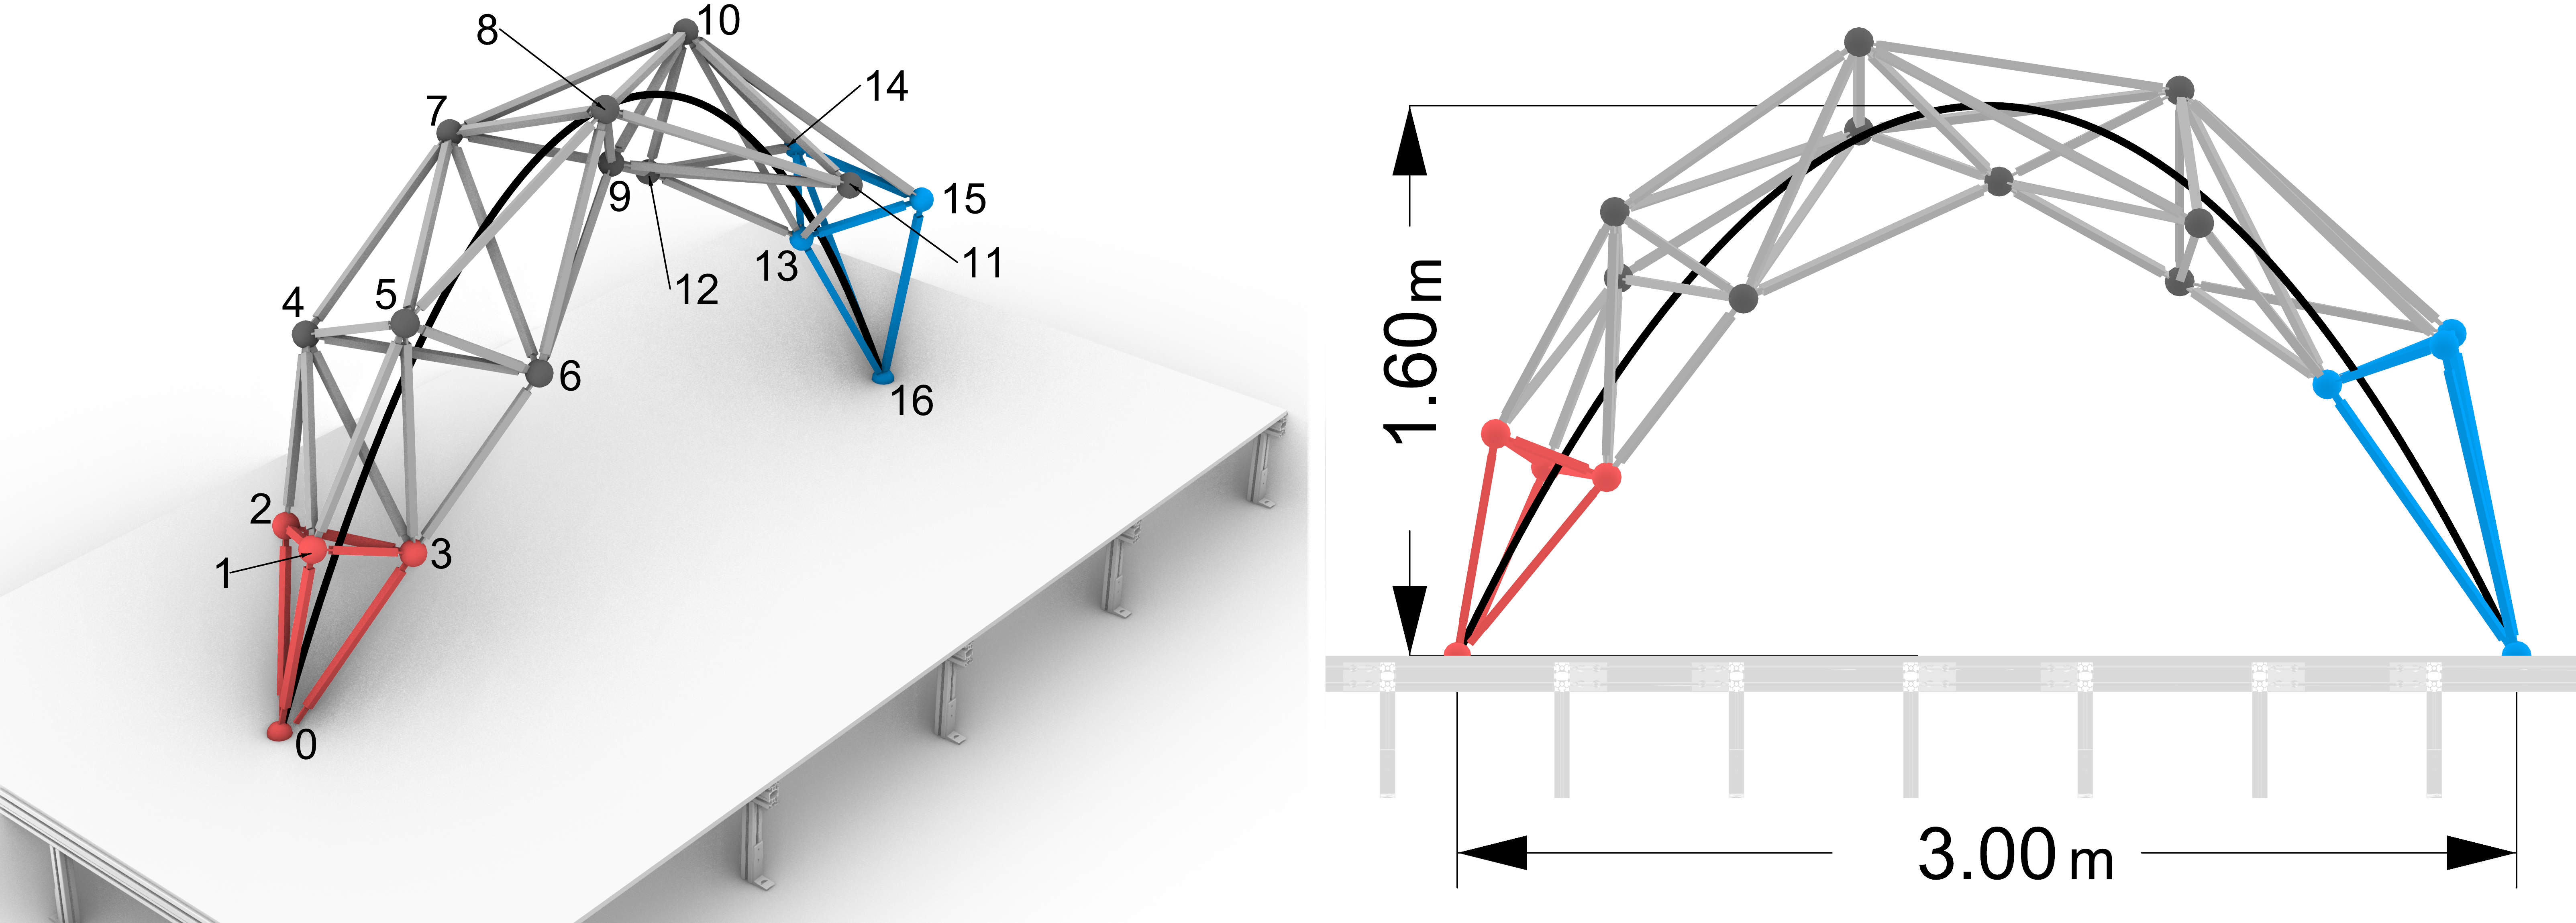
\includegraphics [trim={0cm 0cm 0cm 0cm}, clip, width=0.95\linewidth]{fig7_final_render} %margins tight
    	\caption{Renderings of the designed space frame arch structure showing the node numbers and start/end tetrahedral cells (red/blue).}
    	\label{fig:fig7_final_render} 
    \end{figure}


% ----------------------------------------------------------------------------------------------------
% 5. Disassembly
% ----------------------------------------------------------------------------------------------------
\section{Planning a Cooperative Robotic Disassembly Sequence} \label{sec:5_disassembly}
    When designing a structure for robotic assembly, the emphasis is on allowing for geometric complexity in the design, which can be achieved by placing individual elements to build up a series of rigid cells. In contrast, a disassembly sequence is an operation on a completed structure, and thus a fixed final geometry. Therefore, the resulting process of taking the structure apart can occur through the hybrid removal of existing rigid cells and individual members, to minimize the total number of robotic operations necessary to complete the process. The fewer operations, the faster the full structure can be disassembled.

    Planning the disassembly sequence is presented here based on subtractive operations on the graph representation of the structure. Instead of reducing the graph vertex by vertex, with inverse 3-member Henneberg steps, a more efficient approach is to locate, disconnect and then remove larger locally rigid regions of the graph. These regions correspond to the rigid cells formed in the structure during its design and assembly. The challenge is that their removal must be sequenced such that stability is maintained throughout the full disassembly process. 
    
\subsection{Cooperative Robotic Disassembly Strategy} \label{sec:5__disassemblystrat}
    The approach to disassembly is similar to assembly in that the two robots are sequenced to provide temporary support to the structure while they also actively participate in its sequential disassembly. But although the overall goal of maintaining rigidity at intermediate stages is the same in both assembly and disassembly, the implementation here differs from assembly as performing the removal operation, does not need to occur element by element. 
    
    The disassembly sequence takes advantage of the fact that the structure is specifically designed as a series of nested rigid tetrahedral cells, represented in a planar graph. A sequence can thus be determined where a rigid cell is located, supported, isolated from the rest of the structure, and then independently removed, while preserving the property of rigidity in the stability graph. Having the two robots dedicated to supporting the structure at all times offers more flexibility in this type of disassembly approach as it is now possible to support two distinct regions, and potentially disconnected components, of the structure at all times. 
    
    The process starts by identifying a rigid cell in the structure that is targeted for removal, and assigning a robot to grab and support any member in this cell. Another distinct rigid cell, adjacent to the cell to be removed, is then located in the structure and the second robot is placed there as support. A distinct adjacent cell shares no members with another cell, and is separated by only one member from the cell it is adjacent to. These two cells, $C_{remove}$ and $C_{support}$, are now supported by the two robots, and the edges in the graph between them become redundant from the point of view of minimal rigidity in the stability graph. These edges are effectively locked between two regions of the graph that are rigid when robotic support is provided to them. Thus, the physical members represented by these edges can be removed one by one without compromising either overall stability of the structure or the rigidity of the local region the members are adjacent to. Once the intermediate members are removed, the result is a graph partitioned into two independent rigid components: (1) a disconnected single rigid cell supported by a robot, (2) the remaining structure supported by the other robot and the external foundation support. The single cell can now be removed as a whole component from the work area by the robot supporting it, and the process of disconnection and removal begins again, now starting with the rigid cell that was supported by the other robot (i.e., $C_{support}$ $\rightarrow$ $C_{remove}$). This process is schematically shown in \Cref{fig:disassembly} for a simple 2D truss. 
    
    \begin{figure}[ht]
    	\centering
    	\includegraphics [trim={0cm 0cm 0cm 0cm}, clip, width=0.99\linewidth]{fig11_xmple_disass}
    	\caption{Demonstration of a disassembly sequence where rigid cells are sequentially located, supported, isolated and then removed from a structure.}
    	\label{fig:disassembly} 
    \end{figure}  
    
    Using a cell-by-cell approach allows the full structure to be disassembled with fewer robotic repositioning steps than would be required in a member-by-member approach. Determining which rigid cells to remove and support in each disassembly phase is performed through operations on the isomorphic graph representation -- utilizing the property of planarity and the tetrahedral topology that was explicitly generated in the design process. A non-planar graph would imply a more complex connection hierarchy within the structure, representing sub-structures that are not independently rigid and can therefore not be isolated and removed in a stability-preserving way.
    
    The removal of the intermediate members is done manually, as an example of Human-Robot Interaction (HRI) in a collaborative fabrication process \cite{bruun_humanrobot_2020, han_bridging_2021}. \textit{Collaborative} refers to a process where the human works alongside the robot, while \textit{cooperative} refers to a process where multiple robotic agents work together to accomplish a task one of them alone could not. The task of removing intermediate members is best performed manually, rather than robotically, because spatial accuracy and support capabilities are not required when members can be removed individually without compromising the stability of the structure.
    
\subsection{Algorithm for Locating Rigid Cells} \label{sec:5__algorithm}
    Establishing a feasible disassembly sequence requires locating 1) rigid cells in the structure for the robots to support (\cref{sec:5__algorithm,,sec:5__evaluate}), and 2) intermediate elements to remove (\cref{sec:5__remove}). This procedure is performed through topological computations on the isomorphic planar graph generated from the design process described in \Cref{sec:4__method}. A graph-based algorithm finds rigid cells in the structure, and uses this information when planning a stability-preserving disassembly sequence. The rigid cell locating algorithm is initialized by choosing an edge in the graph to support, and then identifying the corresponding rigid tetrahedral cells to which it belongs. This procedure is described through pseudo-code in \Cref{algo:cell_find} and in greater detail in the remainder of this section. 

    \vspace{1em}
    \begin{algorithm}[ht]
        \setstretch{1.05}
    	\caption{Rigid Tetrahedral Cell Locating Algorithm}
    	\begin{algorithmic}[1]
    	    \State Choose supported edge, $e_{support} = \{v_1, v_2\}$
    	    
    	    \item[]
    		\For {Every $v \in e_{support}$}
		        \State calculate closed neighbourhood graph, $N_G[v_i]$
	        \EndFor
	        \State find common vertices, $V' = N_G[v_1] \ \cap \ N_G[v_2]$
	        
	        \item[]
    		\For {Every $N_G$}
		        \State eliminate edges that are not adjacent to $V'$
		        \State remaining edges, $E_i'$, to form graph, $N_i' = G(V',E_i')$
	        \EndFor
	        \State form adjacent cell subgraph, $N' = N_1' \cup N_2'$
		    
		    \item[]
		    \State calculate complete edge set, $E_f'$
		    \State $E_c'$ = $E_f' - N'$ = edges missing
		    
		    \item[]
    		\For {Every $e \in E_c'$}
		        \State form a tetrahedral cell, $C_i$ by adding, $e_i$, to $N'$
		        \State then remove vertices that are not 3-connected
	        \EndFor
		    
		    \item[]
		    \State evaluate if support member and corresponding tetrahedral cell(s) are adequate to support based on procedure described in \Cref{sec:5__evaluate}
		    \State repeat algorithm until valid cell is located
		    
    	\end{algorithmic}
    	\label{algo:cell_find}
    \end{algorithm} 
    
    Next, the algorithm is further explained with a demonstration of its step-wise execution given an example starting edge, $e_{support} = (11,12)$, operating on the graph generated in \Cref{sec:4_assembly}. This edge is indicated in the graph of the finished space frame arch structure that was designed (\cref{fig:fig9a_support_graph}). The algorithm can be executed given a random edge, or an edge informed by the overall geometry and load-path. This decision is based on the type of structure being disassembled. For example, in a linear structure such as the arch, the disassembly should start from either end of the structure, rather than the middle, so that there are no more than two disconnected regions of the graph at any one time.
    
    \begin{figure}[ht]
    	\centering
    	\includegraphics [trim={0cm 0cm 0cm 0cm}, clip, width=0.99\linewidth]{fig9a_support_graph} %margins tight
    	\caption{Isomorphic planar graph of a space frame arch structure indicating a potential support edge, $e_{support} = (11,12)$, used to initialize the rigid cell finding algorithm.}
    	\label{fig:fig9a_support_graph} 
    \end{figure}   
    
    The process starts with choosing a set of supported edges in $G = (V,E)$, the planar isomorphic graph of the space frame structure. The supported vertices, $V_{support} = \{v_1 \cdots v_n\}$, are adjacent to these edges. For a single supported edge, $n = 2$. A set, $S$, of closed neighborhood graphs is then calculated from each supported vertex in $G$:
    
    \begin{equation}
        S = \{N_G[v] \ | \ v \in V_{support}\} 
    \end{equation}
    
     To simplify the notation, $N_G[v_i] = N_i$. Edges that are not components of the same rigid tetrahedral cells as the supported member must be removed from the neighborhood graphs. First, a subset of common vertices, $V'$, is created across the neighborhood graph vertices:
    
    \begin{equation}\label{eq:2}
        V' = N_1(V) \ \cap \ N_2(V)
    \end{equation}
    
    Next, for each neighborhood graph, $N_i \in S$, a reduced neighborhood subgraph, $N_i' = (V', E_i')$, is created by eliminating edges that are not adjacent to the common vertices in $V'$:  

    \begin{equation}
        E_i' =\{\left(v_i,u\right)\in N_i\ |\ u\in V^\prime\}
    \end{equation}
    
    $N'$, defined as the \textit{adjacent cell subgraph}, is then formed as the union of these reduced neighborhoods:
    
    \begin{equation}
        N' = N_1' \cup N_2'
    \end{equation}    
    
    $N'$ only has vertices and edges that are part of a rigid cell that contains the supported element. Searching for a tetrahedral cell topology, it is evident that there are two potential cells that contain the supported member as seen in \Cref{fig:fig9b_spanning_graph}. But while all the vertices are present, there is one edge missing per cell. 

    \begin{figure}[ht]
    	\centering
    	\includegraphics [trim={0cm 0cm 0cm 0cm}, clip, width=0.99\linewidth]{fig9b_spanning_graph} %margins tight
    	\caption{The adjacent cell subgraph, $N'$, is formed from the union of the reduced support neighborhood subgraphs, $N_1'$ and $N_2'$.}
    	\label{fig:fig9b_spanning_graph} 
    \end{figure} 
    
    The complete edge set, $E_f'$, for the rigid cells containing the supported member, is computed as all edges in the original graph, $G = (V,E)$, adjacent to the common vertices in $V'$:
    
    \begin{equation}
        E_f'=\{(u,v) \in G\ |\ u,v \in V'\}
    \end{equation}
    
    The set of missing edges, $E_c'$, to complete the partial cells in $N'$, is computed as the difference between the full edge set, $E_f'$, and the edges of the \textit{adjacent cell subgraph}:
    
    \begin{equation}\label{eq:missing_edge}
        E_c' = E_f' \ \backslash \ N'(E) = \{e_1 \cdots e_n\}
    \end{equation}
    
    The size of this edge set (i.e., $|E_c'|$) indicates the number of tetrahedral cells containing the supported element. This operation is based on the knowledge that the overall structure is specified to be made up of a series of tetrahedral rigid cells, thus the algorithm is locating as many copies of this specific topology that exist in the neighborhood of the supported member.
    
    The individual subgraphs of each cell are created by first adding each edge, $e_i \in E_c'$, separately to the \textit{adjacent cell subgraph}:
    
    \begin{equation}
        C_i = N'(V, E \cup e_i )
    \end{equation}
    
    Then removing vertices, $v$, in the resulting graph, $C_i$, that are not 3-connected:
    
    \begin{equation}
        C_i = C_i - \{v \ | \ v \in C_i(V) \land deg(v) \neq 3\} 
    \end{equation}
    
    In this example, with $e_{support} = (11,12)$, the result is two cells, $C_1$ and $C_2$, in the overall graph, $G$, that contain the supported edge, shown in \Cref{fig:fig9c_cells_graph}. They have vertex sets $V_{C1} = \{9,10,11,12\}$ and $V_{C2} = \{10,11,12,13\}$, which share three common vertices (i.e., $|V_{C1} \cap V_{C2}|\ =3$) because the cells share a common face.
    
    \begin{figure}[ht]
    	\centering
    	\includegraphics [trim={0cm 0cm 0cm 0cm}, clip, width=0.99\linewidth]{fig9c_cells_graph} %margins tight
    	\caption{Rigid tetrahedral cell subgraphs containing the supported member, $e_{support} = (11,12)$. These cells are computed from the addition of a single edge, $e_i \in E_{c}'$, to the cell adjacency subgraph, and then removing vertices that are not 3-connected.}
    	\label{fig:fig9c_cells_graph} 
    \end{figure} 
    
    It is possible that an edge is only part of one rigid cell (i.e., $|E_c'|\ =\ 1$). The reader can verify this result by following the steps outlined in this section given a different starting support edge (e.g., $e_{support} = (8,11)$). 
    

\subsection{Selecting a Rigid Cell to Support}\label{sec:5__evaluate}
    In each disassembly phase, the current cell being isolated and removed is referred to as $C_{remove}$, and the other supported cell in the structure is referred to as $C_{support}$ (\cref{fig:fig9d_structure_cells}). Once a phase is complete, $C_{support}  \rightarrow C_{remove}$ in the next phase, and the process repeats. The algorithm described in \Cref{sec:5__algorithm} is executed multiple times per phase, varying the supported member initialization to generate an aggregated set of potential rigid cells, $\{C_1 \dots C_n\}$. Naively this requires $|G'(E)|$ runs for a complete characterization of the structure, where $G'$ is a subgraph representing the structure in a partially disassembled state. In practice, this procedure can be reduced significantly as $C_{support}$ must be located adjacent to $C_{remove}$ in the structure. Once the set of rigid cells has been assembled, one cell from here must be chosen as the cell to support in the current phase.
    
    $C_{support}$ is chosen based on the criteria that all intermediate edges connecting it to $C_{remove}$ can be individually removed without breaking apart a non-supported cell in the structure or $C_{remove}$ itself (i.e., compromising rigidity). Thus, the requirement for $C_{support}$ is that it must be immediately adjacent to $C_{remove}$, expressed as the following two conditions:

    \newpage
    \begin{enumerate}
        \item No vertex overlap between $C_{support}$ and $C_{remove}$ (i.e., not too close):
        
        \begin{equation}\label{eq:crit_1}
            C_{support}(V) \cap C_{remove}(V) = \emptyset
        \end{equation}
        
        \item No unsupported vertices between $C_{support}$ and $C_{remove}$ (i.e., not too far):
        \begin{equation}\label{eq:crit_2}
            v\in \{C_{support}(V) \cup C_{remove}(V)\}\ \land \ v\in P
        \end{equation}
    \end{enumerate}
    
    where, $P$, is a set of vertices representing all the possible walks of length two between both cells in the graph.
    
    For example, \Cref{fig:fig9d_structure_cells} illustrates the two rigid cells, $\{C_1,C_2\}$, that are located when initializing the algorithm with $e_{support} = (11,12)$, and the single cell, $C_3$, that is located when initializing the algorithm with $e_{support} = (8,11)$. $C_2$ fails criterion \#1 (\cref{eq:crit_1} as one of the vertices overlaps with $C_{remove}$, thus it cannot be removed as a complete cell without destabilizing the rigid cell $C_2$ by removing one of its vertices. $C_3$ fails criterion \#2 (\cref{eq:crit_2} as supporting this cell leaves a region of the remaining structure directly connected to $C_{remove}$ unsupported. When removing individual members during the disassembly process this unsupported region of the graph is destabilized. Meanwhile, $C_1$ is feasible cell as a robot placed here supports the remaining structure while not leaving any unsupported intermediate vertices connected to $C_{remove}$. Thus, the intermediate members can be manually removed without compromising stability, as each member is immediately adjacent to a rigid supported cell.

    \begin{figure}[H]
    	\centering
    	\includegraphics [trim={0cm 0cm 0cm 0cm}, clip, width=0.90\linewidth]{fig9d_structure_cells}
    	\caption{Checking the viability of a rigid cell to support in relation to the location of the current cell being removed. $C_1$ is a valid cell to support, while $C_2$ and $C_3$ violate the adjacency criteria.}
    	\label{fig:fig9d_structure_cells} 
    \end{figure} 

    
\subsection{Selecting Individual Members to Remove} \label{sec:5__remove}
    Once a viable rigid cell to support is chosen based on the criteria outlined in \Cref{sec:5__evaluate}, the set of edges, $E_{remove}$, that connect $C_{remove}$ and $C_{support}$, is computed as per \Cref{eq:remove_edge}. $G'$ is the graph of the full structure in the current disassembly phase. Following the removal of the intermediate members in any order, the cell $C_{remove}$ is disconnected from the remaining structure and is removed as an independent component.

    \begin{equation}\label{eq:remove_edge}
        E_{remove} = \{(u,v) \in G' \ | \ u \in C_{remove}, v \in C_{support}\}
    \end{equation}
    

\subsection{Planning the Disassembly Sequence for a Spanning Space Frame Arch} \label{sec:5__casestudy}
    Computing a stability-preserving disassembly sequence using two robots is implemented on the space frame structure designed in \Cref{sec:4__casestudy}. The complete disassembly of the structure is found to only require four phases. Each phase starts with the repositioning of a robot to support a viable rigid cell, $C_{support}$, located as per \Cref{sec:5__algorithm,sec:5__evaluate}, and ends with the removal of a set of intermediate members, $E_{remove}$ as per \Cref{sec:5__remove}, followed by the removal of $C_{remove}$. \Cref{table:disassembly} summarizes the key information computed for each phase, where $G'$ is the graph of the remaining structure at the start of each disassembly phase. $G'_{end}$ shows the results of the algorithm operating on $G'$, with the location of $C_{remove}$ in blue, $C_{support}$ in red, and $E_{remove}$ in green. The vertex and edge sets for each of these components are listed in the table for each phase.
    
    The process starts by choosing $C_{remove}$ as the rigid cell at one end of the arch, and progresses over the whole structure, with $C_{support} \rightarrow C_{remove}$ in the following phase.

    \def\colpicwidth{0.20}
    \setcellgapes{0pt}
    
    \begin{table}[ht]
    	\renewcommand{\arraystretch}{1.2}
    	\scriptsize
    	\centering
    	\caption{The four disassembly phases planned for the arch structure designed in \Cref{sec:4__casestudy}.}
    	% \vspace{-2.5mm}
    	
    	\begin{tabular}{m{1.2cm} m{0.1cm} m{\colpicwidth\textwidth} m{2.1cm}m{2.1cm}p{1.0cm} m{\colpicwidth\textwidth}}
    		\specialrule{.10em}{0.2em}{.2em}
    		\centering
    		%
    		\phantom{a}%to space out the top headings nice
    		&\phantom{\makecell{\vspace{0.5em}}}%to space out the top headings nice
    		&\multicolumn{1}{c}{\small{$G'$}}
    		&\multicolumn{1}{c}{\textcolor{SkyBlue}{\small{$C_{remove}$}}}
    		&\multicolumn{1}{c}{\textcolor{Salmon}{\small{$C_{support}$}}}
    		&\multicolumn{1}{c}{\textcolor{OliveGreen}{\small{$E_{remove}$}}}
    		&\multicolumn{1}{c}{\small{$G'_{end}$}}
    		\\	
    		\specialrule{0.06em}{0.2em}{.2em}
    		%
    		\small{Phase 1}
    		&& \includegraphics [trim={0cm 0cm 0cm 0cm}, clip, width=\colpicwidth\textwidth]{fig10_p1_1}
    		& \scriptsize{\makecell[cb]{V = \{13,14,15,16\} \\ \\ E = \{\\(13,14)\\(13,15)\\(13,16)\\(14,15)\\(14,16)\\(15,16)\}}}%
    		& \scriptsize{\makecell[cb]{V = \{9,10,11,12\} \\ \\ E = \{\\(9,10)\\(9,11)\\(9,12)\\(10,11)\\(10,12)\\(11,12)\}}}%
    		& \scriptsize{\makecell[cc]{\phantom{V = 1} \\ \\ E = \{\\(10,13)\\(10,14)\\(10,15)\\(11,13)\\(12,13)\\(12,14)\}}}
    		& \includegraphics [trim={0cm 0cm 0cm 0cm}, clip, width=\colpicwidth\textwidth]{fig10_p1_2}\\
    		%
    		\\ \cmidrule{1-7} \\
    		%
    		\small{Phase 2}
    		&& \includegraphics [trim={0cm 0cm 0cm 0cm}, clip, width=\colpicwidth\textwidth]{fig10_p2_1}
    		& \scriptsize{\makecell[cb]{V = \{9,10,11,12\} \\ \\ E = \{\\(9,10)\\(9,11)\\(9,12)\\(10,11)\\(10,12)\\(11,12)\}}}%
    		& \scriptsize{\makecell[cb]{V = \{5,6,7,8\} \\ \\ E = \{\\(5,6)\\(5,7)\\(5,8)\\(6,7)\\(6,8)\\(7,8)\}}}%
    		& \scriptsize{\makecell[cc]{\phantom{V = 1}  \\ \\ E = \{\\(6,9)\\(7,10)\\(7,9)\\(8,9)\\(8,10)\\(8,11)\}}}
    		& \includegraphics [trim={0cm 0cm 0cm 0cm}, clip, width=\colpicwidth\textwidth]{fig10_p2_2}\\
    		%
    		\\ \cmidrule{1-7} \\
    		%
    		\small{Phase 3}
    		&& \includegraphics [trim={0cm 0cm 0cm 0cm}, clip, width=\colpicwidth\textwidth]{fig10_p3_1}
    		& \scriptsize{\makecell[cb]{V = \{5,6,7,8\} \\ \\ E = \{\\(5,6)\\(5,7)\\(5,8)\\(6,7)\\(6,8)\\(7,8)\}}}%
    		& \scriptsize{\makecell[cb]{V = \{1,2,3,4\} \\ \\ E = \{\\(1,2)\\(1,3)\\(1,4)\\(2,3)\\(2,4)\\(3,4)\}}}%
    		& \scriptsize{\makecell[cc]{\phantom{V = 1} \\ \\ E = \{\\(1,5)\\(3,6)\\(4,5)\\(4,6)\\(4,7)\\(5,6)}}
    		& \includegraphics [trim={0cm 0cm 0cm 0cm}, clip, width=\colpicwidth\textwidth]{fig10_p3_2}\\
    		%
    		\\ \cmidrule{1-7} \\
    		%
    		\small{Phase 4}
    		&& \includegraphics [trim={0cm 0cm 0cm 0cm}, clip, width=\colpicwidth\textwidth]{fig10_p4_1}
    		& \scriptsize{\makecell[cb]{V = \{1,2,3,4\} \\ \\E = \{\\(1,2)\\(1,3)\\(1,4)\\(2,3)\\(2,4)\\(3,4)\}}}%
    		& \scriptsize\makecell[cb]{{$-$}}%
    		& \scriptsize{\makecell[cc]{E = \{\\(0,1)\\(0,2)\\(0,3)}}
    		& \includegraphics [trim={0cm 0cm 0cm 0cm}, clip, width=\colpicwidth\textwidth]{fig10_p4_2}\\
    		%
    		\specialrule{0.10em}{0.2em}{.2em}
    		%
    	\end{tabular}
    	
    	\label{table:disassembly}
    \end{table}        


% ----------------------------------------------------------------------------------------------------
% 6. Results
% ----------------------------------------------------------------------------------------------------
\clearpage
\section{Assembly and Disassembly Results and Discussion} \label{sec:6_results}

\subsection{Space Frame Assembly} \label{sec:6__assembly}
    The 17-noded space frame structure, designed for the target $3.0 m \times 1.6 m$ arch geometry in \Cref{sec:4__casestudy}, is physically assembled in the Embodied Computation Lab lab at Princeton University. This is done using a robotic cell comprised of two ABB IRB4600-40/2.55 robotic arms on 3.9 m linear tracks. The purpose of this exercise is to validate the design method presented in this chapter and to test the rigidity-preserving cooperative robotic fabrication sequence that the structure is designed for. The material system used for the structure is 85 mm diameter 3D-printed PETG hollow nodes (with embedded slots for the member connection tabs) and 30 mm square wood members, which are fastened manually with 6mm machine screws drilled through a 3D-printed tapered PETG tab inserted through a slot at each member's end. This tabs acts as the connector between the member and the node, and is itself manually placed after the member is maneuvered to the correct location with the robotic arm, which is instrumented with a pneumatic gripper (\cref{fig:structure_fabricate}).
    
    \begin{figure}[h]
    	\centering
    	\begin{subfigure}[b]{0.49\linewidth}
    		\centering
    		\includegraphics [trim={0cm 0cm 0cm 0cm}, clip, width=1\textwidth]{structure_node}
    	\end{subfigure}
        %
    	\begin{subfigure}[b]{0.49\linewidth}
    		\centering
    		\includegraphics [trim={0cm 0cm 0cm 0cm}, clip, width=1\textwidth]{structure_gripper}
    	\end{subfigure}    
    	\caption{A typical structural node with connecting tabs (left). A robotic arm with pneumatic gripper placing and supporting a member in the structure (right).}
    	\label{fig:structure_fabricate} 
    \end{figure}
    
    Snapshots of the structure, and its corresponding stability graph, as examples of the assembly process are shown in \Cref{fig:fig8_during_construction} during the execution of a 3-member aggregation sequence for nodes 7 and 11. \Cref{fig:fig8_a,,fig:fig8_b} show the structure during a partially completed Henneberg sequence for node 7, where only two of the three members have been placed and the structure is supported by both robots: $e_{support} = \{(4,7),(5,7)\}$. \Cref{fig:fig8_c,,fig:fig8_d} show the stage where node 11 is fully connected and the structure itself becomes minimally rigid (i.e., at the end of a Henneberg 3-member sequence), with support from one robot only required for overall stability: $e_{support} = \{(10,11)\}$. The full fabrication sequence is shown in Appendix A, \Cref{table:appendix_sequence}, which summarizes the order of assembly, the edge in the graph each member corresponds to, and the robot ($R1$ or $R2$) that was used to place a member as part of a 3-member sequence. The finished structure is shown in \Cref{fig:final_structure}.

    \begin{figure}[ht]
    	\centering
    	\begin{subfigure}[b]{0.55\linewidth}
    		\centering
    		\includegraphics [trim={0cm 0cm 0cm 0cm}, clip, width=0.99\textwidth]{structure_support2}
    		\caption{both robots supporting the structure in a partially completed Henneberg Type 1 step for node 7.}
    		\label{fig:fig8_a}
    	\end{subfigure}
        %
    	\begin{subfigure}[b]{0.44\linewidth}
    		\centering
    		\includegraphics [trim={0cm 0cm 0cm 0cm}, clip, width=0.99\textwidth]{fig8_temp_graph_1}
    		\caption{rigid stability graph of the structure showing the 4 supported vertices in red.}
    		\label{fig:fig8_b}
    	\end{subfigure}
    	
    	\vspace{1em}
    	
    	\begin{subfigure}[b]{0.55\linewidth}
    		\centering
    		\includegraphics [trim={0cm 0cm 0cm 0cm}, clip, width=0.99\textwidth]{structure_support1}
    		\caption{a single robot supporting the structure after a completed Henneberg Type 1 step for node 11.}
    		\label{fig:fig8_c}
    	\end{subfigure}
        %
    	\begin{subfigure}[b]{0.44\linewidth}
    		\centering
    		\includegraphics [trim={0cm 0cm 0cm 0cm}, clip, width=0.99\textwidth]{fig8_temp_graph_2}
    		\caption{rigid stability graph of the structure showing the 3 supported vertices in red.}
    		\label{fig:fig8_d}
    	\end{subfigure}
    	%
    	\caption{Snapshots of the cooperative robotic assembly process for the space frame arch structure. Robotic support is shown on the structure and its isomorphic graph for a partially completed (top) and completed (bottom) 3-member Henneberg sequence.}
    	\label{fig:fig8_during_construction} 
    \end{figure}

    \begin{figure}[ht]
    	\centering
    	\includegraphics [trim={0cm 0cm 0cm 0cm}, clip, width=0.99\linewidth]{final_structure}
    	\caption{The 17-noded space frame arch structure as the realization of a planar graph designed to have a rigidity-preserving (dis)assembly sequence.}
    	\label{fig:final_structure} 
    \end{figure}   

    \newpage
    The robotic fabrication sequence for the full structure is planned using the COMPAS FAB framework \citep{mele_compas_2017} to calculate feasible collision-free paths for the robots to take while placing members. For a geometrically complex structure, individual members can be more easily maneuvered in space by the robots, which improves the likelihood of a feasible collision-free path to be found. But even so, as assembly progresses and the structure grows in size, it becomes more difficult to find feasible collision-free paths. To help with the path planning process in later stages of assembly, the calculation of trajectories is split into two discrete planning operations: (1) from the fixed pick-up location to an unobstructed intermediate plane in space; (2) from the intermediate plane to the final location of the member, also expressed as a plane located at the member's geometric center. The intermediate plane is located approximately 500 mm away from the structure and is parallel to the member's final location plane, which is based on the cartesian position and orientation taken from an accurate 3D model of the structure. The likelihood of a feasible path being calculated is improved as the first operation would maneuver the robot in unobstructed space to a position in line with the member's final location, and the second operation would perform a relatively simple linear cartesian move to the final location. The control of the robots, and execution of the calculated trajectories for the placement of each member, is then done using the COMPAS RRC framework \citep{fleischmann_compas_2020}. Placement errors (i.e., positional differences between the digital model and as-built structure) ranged from 1-10 mm between the end of members and connection slots in the nodes. This was within the tolerance of the material system, therefore no correction using sensors or 3D imaging (as in \citep{ding_bim-based_2020}) was required during construction.

    The rigidity-preserving assembly logic, and the resultant structure designed using the method developed in this chapter, is specifically based around the use of two robotic arms. Adding an additional robotic support agent to the setup would greatly expand the design space for rigidity-preserving space frame structures, by allowing more complex cooperative robotic sequences to be performed. For example, it would be possible to construct rigid cells composed of five or six vertices, rather than the four as in the tetrahedral cell. These rigid cells can be realized through more complex rigidity-preserving fabrication sequences based on combinations of both Henneberg Type 1 and 2 steps. The ability to build cells with six vertices is particularly promising as there are four different rigid topological configurations that are possible, which would thus allow for additional flexibility during the design stage. Finally, a third robotic agent would allow for a more complex load-path, allowing for stable branching structures to be built beyond the linear partial order that is currently possible with two robots. 



\subsection{Space Frame Disassembly}\label{sec:6__disassembly}
    The disassembly sequence computed in \Cref{sec:5__casestudy} is implemented on the completed structure at the end of the assembly sequence (\cref{fig:final_structure}). The results of the physical implementation of this rigidity-preserving sequence are documented for each of the four phases in \Cref{table:disassembly_images}. The left column shows the disconnected structure, with one robot supporting the rigid tetrahedral cell to remove ($C_{remove}$) and the other robot supporting the remaining rigid portion of the arch structure. The right column shows close-up images of the rigid cell and the six intermediate members removed ($E_{remove}$) in the process of disconnecting the cell from the rest of the structure.

    \def\colpicwidth{0.37}
    \setcellgapes{0pt}
    
    \begin{table}[H]
    	\renewcommand{\arraystretch}{1.0}
    	\small
    	\centering
    	\caption{Documentation of the four phases of the rigidity-preserving disassembly sequence calculated and executed for the space frame arch structure.}
    	% \vspace{-2.5mm}
    	
    	\begin{tabular}{m{1.2cm} p{0.1cm} m{\colpicwidth\textwidth}m{\colpicwidth\textwidth}}
    		\specialrule{.10em}{0.2em}{.2em}
    		\centering
    		%
    		\phantom{a}%to space out the top headings nice
    		&\phantom{\makecell{\vspace{0.5em}}}%to space out the top headings nice
    		&\multicolumn{1}{c}{\normalsize{Disconnected Supported Structure}}
    		&\multicolumn{1}{c}{\normalsize{$C_{remove}$ and $E_{remove}$}}
    		\\
    		\specialrule{0.06em}{0.2em}{.2em}
    		%
    		Phase 1
    		&& \includegraphics [trim={0cm 0cm 0cm 0cm}, clip, width=\colpicwidth\textwidth]{disassemble_p1}
    		& \includegraphics [trim={0cm 0cm 0cm 0cm}, clip, width=\colpicwidth\textwidth]{disassemble_p1_2}\\
    		%
    		\cmidrule{1-4}
    		%
    		Phase 2
    		&& \includegraphics [trim={0cm 0cm 0cm 0cm}, clip, width=\colpicwidth\textwidth]{disassemble_p2}
    		& \includegraphics [trim={0cm 0cm 0cm 0cm}, clip, width=\colpicwidth\textwidth]{disassemble_p2_2}\\
    		%
    		\cmidrule{1-4}
    		%
    		Phase 3
    		&& \includegraphics [trim={0cm 0cm 0cm 0cm}, clip, width=\colpicwidth\textwidth]{disassemble_p3}
    		& \includegraphics [trim={0cm 0cm 0cm 0cm}, clip, width=\colpicwidth\textwidth]{disassemble_p3_2}\\
    		%
    		\cmidrule{1-4}
    		%
    		Phase 4
    		&& \includegraphics [trim={0cm 0cm 0cm 0cm}, clip, width=\colpicwidth\textwidth]{disassemble_p4}
    		& \includegraphics [trim={0cm 0cm 0cm 0cm}, clip, width=\colpicwidth\textwidth]{disassemble_p4_2}\\
    		%
    		\specialrule{0.10em}{0.2em}{.2em}
    		%
    	\end{tabular}
    	
    	\label{table:disassembly_images}
    \end{table}     

    \newpage
    The computation of the disassembly sequence does not provide information about which of the six elements comprising each selected cell a robot should support. While this choice does not impact rigidity (i.e., any of the six elements are valid), an additional finite element analysis was performed to inform which robot should support which cell in each phase, and the optimal combination of supported elements in each of the two cells ($C_{remove}$ and $C_{support}$). The combination of supported elements that result in the minimum average strain energy during the full disassembly process in each phase are summarized in \Cref{table:disassembly_results}. The methodology for this analysis and the full data for all possible support combinations in each phase are shown in Appendix B. Robotic reachability also impacts which members can be supported, but is not an issue in this specific case as most members are within reach of at least one robot, which is verified using the path-planning functionality in COMPAS FAB \citep{mele_compas_2017}. In general, supporting members that are located close to the central axis of the arch results in lower average axial strain energy in the structure, for all steps in a particular disassembly phase. This result is due to the structure experiencing less out-of-plane twisting when supported at these central locations.

    \begin{table}[h]
    	\renewcommand{\arraystretch}{1.2}
    	\small
    	\centering
    	\caption{The two members supported by either robot resulting in the minimum average axial strain energy ($10^{-9} \ kN\cdot m$) in each disassembly phase.}
    	% \vspace{-2.5mm}
    	
    	\begin{tabular}{m{1.4cm} m{2.5cm}m{2.5cm}p{1.5cm}}
    		\specialrule{.10em}{0.2em}{.2em}
    		\centering
    		%
    		\phantom{a}%to space out the top headings nice
    		&\multicolumn{1}{c}{\normalsize{$R_1$}}
    		&\multicolumn{1}{c}{\normalsize{$R_2$}}
    		&\multicolumn{1}{c}{\normalsize{$E_{\epsilon,avg}$}}
    		\\	
    		%
    		\specialrule{0.06em}{0.2em}{.2em}
    		%
    		Phase 1
    		& \makecell[cb]{$C_{support}$ \\[-0.5em] \\[-0.5em] member = 31  \\[-0.5em] \\[-0.5em]  e = (11,12)}%
    		& \makecell[cb]{$C_{remove}$  \\[-0.5em] \\[-0.5em]  member = 41  \\[-0.5em] \\[-0.5em]  e = (14,15)}%
    		& \makecell[cc]{9.51}
            \\
            \cmidrule{1-4}
            %
    		Phase 2
    		& \makecell[cb]{$C_{support}$  \\[-0.5em] \\[-0.5em]  member = 15  \\[-0.5em] \\[-0.5em] e = (5,7)}%
    		& \makecell[cb]{$C_{remove}$  \\[-0.5em] \\[-0.5em] member = 31  \\[-0.5em] \\[-0.5em] e = (11,12)}%
    		& \makecell[cc]{4.42}
            \\
    		\cmidrule{1-4}
            %
    		Phase 3
    		& \makecell[cb]{$C_{support}$  \\[-0.5em] \\[-0.5em]  member = 6 \\[-0.5em] \\[-0.5em]  e = (1,4)}%
    		& \makecell[cb]{$C_{remove}$  \\[-0.5em] \\[-0.5em] member = 16 \\[-0.5em] \\[-0.5em]  e = (6,7)}%
    		& \makecell[cc]{1.55}
            \\
    		\cmidrule{1-4}
            %
    		Phase 4
    		& \makecell[cb]{$C_{remove}$  \\[-0.5em] \\[-0.5em]  member = 6  \\[-0.5em] \\[-0.5em]  e = (1,4)}%
    		& \makecell[cb]{-}%
    		& \makecell[cc]{0.87}
            \\
    		\specialrule{0.10em}{0.2em}{.2em}
    		%
    	\end{tabular}
    	
    	\label{table:disassembly_results}
    \end{table} 
    
    Using a closed-form algorithm to locate and isolate rigid cells in a structure  during disassembly, such as the one presented in \Cref{sec:5__algorithm}, is a valid approach when given a structure with a uniform topology. For example, as with the example presented in this chapter, where the structure is known to be composed of tetrahedral cells. But a more generic method is necessary when expanding the feasible design space to include structures composed of both more complex and varied rigid cells, and branching load paths (i.e., not a linear partial order of rigid cells). With the future inclusion of a third robotic agent in the fabrication setup, assembling such structures will be possible. The calculation of a feasible rigidity-preserving disassembly sequence must thus be generalized for use in such structures with unknown and varied topologies by developing a more generic approach to the cell locating and isolating algorithm. This will be accomplished in future work through the implementation of a graph-search approach based on the rigidity-finding \textit{pebble game} algorithm \citep{jacobs_algorithm_1997}.
    
    
% ----------------------------------------------------------------------------------------------------
% 7. Conclusions
% ----------------------------------------------------------------------------------------------------
\section{Conclusion} \label{sec:7_conclusion}
    In this chapter, a novel graph theoretic approach, based on rigidity theory, is presented as a way to assess the stability of spatially complex bar and joint structures (i.e., trusses and space frames) during any phase of their construction. A topological framework, referred to as a \textit{stability graph}, is developed as an isomorphic representation of the physical structure (i.e., there exists a one-to-one mapping between the graph and structure). The structural elements, support conditions, and temporary robotic supports can all be represented in the \textit{stability graph}, and their collective effect on the stability of the structure can thus be evaluated using only graph rigidity principles (e.g., Laman count and Henneberg construction steps).
    
    A schematic design method, based on a topology-driven approach to rigidity and structural stability, is then developed. The method is used to design space frame structures that remain stable during all stages of their assembly and disassembly without requiring external scaffolding. The design method is \textit{fabrication-informed}, because it is specifically developed to take advantage of the fabrication capabilities (with respect to sequencing) when two industrial robotic arms work together in a cooperative manner: placing elements (during assembly), removing cells (during disassembly), while also supporting the structure in its temporary state.
    
    The proposed method is demonstrated in this chapter through the design, and robotic assembly and disassembly, of a rigidity-preserving space frame arch, composed of 17 nodes and 45 elements. The structure is sequentially designed to be assembled element-by-element with two robots, mirroring a Henneberg rigid-graph assembly step in the topological design space of the \textit{stability graph}. The design process and assembly logic guarantee that the property of planarity is maintained in the graph, which physically corresponds to a structure that is composed of a series of rigid tetrahedral cells. The property of planarity, coupled with a tetrahedral cell topology, results in a structure that can then also be efficiently disassembled through the application of a graph-based algorithm to sequentially locate and isolate rigid cells in the graph. After the cells are located, they are robotically supported and removed from the physical structure as independent components, all while the stability of the remaining structure is preserved. 
    
    As robotic technology improves, its applications in the AEC industry will continue to grow, with multi-robot setups becoming more prevalent. Engineers and architects should consider how the structures they design can better take advantage of the potential afforded them through such robotic fabrication setups. The generic support/place sequencing approach, that is demonstrated with two robots in this chapter, can help to further expand the feasible design space for geometrically complex discrete element structures. Future work will integrate feedback in the form of 3D imaging of the structure during assembly or disassembly to allow the fabrication process to better adapt to changing conditions such as deformation of the structure due to self-weight. Overall, the goal is to further promote the application of robotic fabrication and automation in construction, while simultaneously improving the material use and construction efficiency of geometrically complex trusses and space frames.

% ----------------------------------------------------------------------------------------------------
% Bibliography
% ----------------------------------------------------------------------------------------------------  
\newpage
\bibliographystyle{\BiblioPath/elsarticle-num} 

\begingroup
    \hypersetup{hidelinks} %turns off colors for URL and DOIs
    \bibliography{\BiblioPath/5SpaceFrame}
\endgroup